\documentclass{svproc}
%
\usepackage{graphicx}%
\usepackage{multirow}%
\usepackage{amsmath,amssymb,amsfonts}%
\usepackage{mathrsfs}%
\usepackage[title]{appendix}%
\usepackage{xcolor}%
\usepackage{textcomp}%
\usepackage{manyfoot}%
\usepackage{booktabs}%
\usepackage{algorithm}%
\usepackage{algorithmicx}%
\usepackage{algpseudocode}%
\usepackage{listings}%
\usepackage{url}
\def\UrlFont{\rmfamily}

\renewcommand{\topfraction}{.99}
\renewcommand{\dbltopfraction}{.99}
\renewcommand{\bottomfraction}{.99}
\renewcommand{\textfraction}{.01}
\renewcommand{\floatpagefraction}{0.9}
\renewcommand{\dblfloatpagefraction}{0.9}

\usepackage[normalem]{ulem}
\usepackage{bm}
\usepackage{xspace}
\usepackage{subcaption}

\usepackage{color}
\def\green#1{\textcolor[rgb]{0,0.6,0}{#1}}
\def\black#1{\textcolor[rgb]{0,0,0}{#1}}
\def\dgreen#1{\textcolor[rgb]{0.02,0.50,0.05}{#1}}
\def\gray#1{\textcolor[rgb]{0.5,0.5,0.7}{#1}}
\def\red#1{\textcolor{red}{#1}}
\def\blue#1{\textcolor{blue}{#1}}
\def\Blue{\color[rgb]{0,0,1}}
\def\Red{\color[rgb]{1,0,0}}
\def\Dgreen{\color[rgb]{0.02,0.55,0.04}}
\def\Black{\color[rgb]{0,0,0}}
\def\ignore#1{}

\usepackage[normalem]{ulem}
\usepackage{bm}
\usepackage{booktabs}
\usepackage{xspace}
\usepackage{subcaption}

% track-changes helpers (kept from last year's setup)
\newcommand{\add}[1]{\textcolor{blue}{#1}}
\newcommand{\erase}[1]{\textcolor{red}{\sout{#1}}}
\def\subst#1#2{\add{#1}{ \erase{#2}}}

% parameters definition (same convention as docs/journal.tex)
\def\post{\rho}                 % posting probability
\def\BoundedConfidence{\epsilon} % bounded confidence (rejection) threshold
\def\feed{F}                    % feed
\def\Stubbornness{\mu}           % stubbornness
\def\maxfollower{S_{\it fol}}    % max followee capacity
\def\maxfeed{S_{\it fd}}         % feed capacity
\def\VCR{\kappa}                 % vocal comfort radius (expression threshold)

\begin{document}
\mainmatter

\title{Moderate Hubs Beyond Direct Transmission: How Homophily and the Spiral of Silence Shape Downstream Opinion Dynamics}
\titlerunning{Moderate Hubs, Homophily, and the Spiral of Silence}

\author{Tomoya Takeda\inst{1}, Fujio Toriumi\inst{2}, Toshiharu Sugawara\inst{1}}
\authorrunning{Tomoya Takeda, Fujio Toriumi and Toshiharu Sugawara} % abbreviated author list (for running head)

\institute{Department of Computer Science and Communications Engineering,
\\Waseda University, 3-4-1 Okubo, Shinjyuku-ku, 169-8555, Tokyo, Japan.\\
\email{tomoya.leo9@fuji.waseda.jp}, \email{sugawara@waseda.jp}
\and
Department of Systems Innovation, The University of Tokyo, \\7-3-1
Hongo, Bunkyo-ku, 113-8656, Tokyo, Japan.\\
\email{tori@sys.t.u-tokyo.ac.jp}
}

\maketitle

\begin{abstract}\Dgreen
With the rapid expansion of web communication platforms, hub users
have become critical actors in online opinion dynamics, yet their
effects on polarized posting behavior remain poorly understood. Using
an agent-based model on heavy-tailed adaptive social networks, we
study how moderate-stanced hubs shape opinion-sharing
behavior. Active moderate hubs consistently boost moderate-camp
posting while suppressing near-extreme posting. 
Their effect on the ideologically distant extreme camp, however, 
is indirect and can reverse across network conditions. 
We trace this sign reversal to a two-layer mechanism combining
homophily, which determines which near-extreme content reaches
extreme agents, and a spiral-of-silence-style expression threshold,
which determines how that content affects their posting.
Our results suggest that the role of 
moderate hubs extends beyond direct transmission: 
content flows regulated by moderate hubs 
can have qualitatively different effects downstream 
through the interaction of network-level filtering 
and agent-level evaluation.
\ignore{With the rapid expansion of web communication platforms, hub users have become critical actors in online opinion expression dynamics; however, their effects on polarized posting behavior remain poorly understood. Using an agent-based model on heavy-tailed adaptive social networks, we study how moderately positioned hubs shape opinion-sharing behavior. Across a comprehensive suite of experiments, we observe a consistent pattern in which active moderate hubs boost moderate-camp posting while suppressing near-extreme posting. Their influence on the ideologically distant extreme camp, however, is highly complex: moderate hubs can act as mediators or facilitators of activation depending on network conditions. We trace this regime shift to a two-layer homophily mechanism, structural and perceptual, which determines whether the two camps are perceived as one group (mediation) or as separate communities (facilitation). Moderate hubs are therefore not universally stabilizing bridges; their brokerage role flips between mediation and facilitation depending on how homophilic the two camps are perceived to be.}
\Black
\keywords{Social networks, Opinion dynamics, Agent-based simulation,
  Social media, Computational Social Science} 
\end{abstract}

\Blue


\section{Introduction}\label{sec:intro}
Social media and web communication platforms have become the primary
venues for various styles of speech and discussion, 
thereby exerting a significant effect on
public opinion formation. Unlike traditional face-to-face
communication, hub users or influencers 
can create posts that are disproportionately amplified
across a platform's population, giving them immense influence on a
given opinion environment. The role and effect of these hubs have been
well studied,
particularly from the perspective of information diffusion. 
However, their consequences for polarized opinion dynamics 
remain less well understood, particularly when 
structurally prominent users themselves occupy 
moderate rather than strongly identified positions.
\par

\Dgreen
As a topic becomes increasingly controversial, popular figures 
whose positions remain moderate along the relevant 
opinion dimension may enter the discussion, 
yet the consequences of their engagement 
remain poorly understood.
Therefore, we investigate how differently polarized posting dynamics
emerge by the sharing activity of moderate hubs.
Using an
agent-based model on heavy-tailed adaptive social networks, we find
that moderate hubs have consistent effects within their direct reach:
they increase posting in the aligned moderate camp while suppressing
posting in the neighboring near-extreme camp. In contrast, their effect
on the ideologically distant extreme camp is indirect and can reverse
depending on the recipients' propensities.
This downstream effect arises because moderate hubs alter the
vocality and resulting information flow of near-extreme agents, rather
than directly reaching the extreme camp. The resulting near-extreme
content is then filtered at two levels: homophily determines
which content reaches extreme agents, while a spiral-of-silence-style
expression threshold determines which of the received content is
sufficiently comfortable to promote vocalization. Their interaction therefore determines whether
the downstream effect of moderate-hub activity facilitates or suppresses
extreme posting.

\par

Our results suggest that the downstream influence of moderate hubs 
on posting dynamics extends beyond
direct transmission: by altering the dynamics within their reach, they
reshape information flows beyond it, but the effects are transformed
rather than simply transmitted as they encounter downstream populations
with different dispositions. 
\Blue

\section{Related Work}\label{sec:related}
Although social networks have long been studied as static structures,
most notably in seminal work on small-world topology~\cite{watts1998},
they have recently been modeled as systems whose topology coevolves
with the opinions and behaviors of the individuals embedded in
them. Building on the classic \emph{voter model}~\cite{clifford1973},
Vazquez et al.~\cite{vazquez2008} used an {\em agent-based model}
(ABM) to analyze coevolutionary dynamics based on two coupled rules
--- state updating and edge rewiring --- revealing a phase transition
between connected and fragmented networks governed by degree
settings. The study of opinion dynamics is one of the major fields
where this style of coevolving network model has been fruitfully
applied: Kozma and Barrat~\cite{kozma2008} modeled how agents
adaptively rewire their social ties in response to disagreement,
showing the dominant effect of homophilic rewiring on the resulting
network structure. This coevolving network model is based on {\em bounded
confidence}, formalized by Deffuant et al.~\cite{deffuant2000} and
Hegselmann and Krause~\cite{hegselmann2002}, in which an agent updates
its opinion only by averaging with others whose opinion falls within a
fixed tolerance window. With the rapid proliferation of social media
in recent years, public discourse has shifted significantly from
traditional face-to-face communication. In line with this
homophilic-rewiring mechanism, Sasahara et al.~\cite{sasahara2020}
used an ABM to confirm that social influence combined with the
unfollowing process successfully reproduces the politically polarized
follow network observed in real-world social media
data~\cite{conover2011}.
\par


Whether such bridging roles are inherently stabilizing, however, is
far from settled in the context of social media. Classic network
theory established that ties bridging otherwise disconnected
communities act as a source of connectivity and innovation rather than
redundancy, whether characterized as \emph{weak ties} diffusing
influence across group boundaries~\cite{granovetter1973} or as
\emph{broker} nodes spanning structural holes~\cite{burt1992}. This
bridging role was later quantified via \emph{betweenness
centrality}~\cite{freeman1977}. On social media,
however, this integrative reading does not hold unconditionally: Cha
et al.~\cite{cha2010} observed that highly followed users do not
necessarily exert a larger influence, 
% which is an important caveat for
% influence maximization in social media marketing --- 
and subsequent studies have shown that
the consequences of hub activity depend on how influence interacts with
opinion dynamics.
Using an ABM, Helfmann
et al.~\cite{helfm2023} showed that hub users who adopt extreme
attitudes can gain more followers on social media. Also with an ABM,
Betts et al.~\cite{betts2023} found that, unlike an extremist
influencer whose activity always accelerates polarization, a neutral
influencer's effect inverts with how broadly it is trusted: narrowly
trusted, it backfires and increases polarization; broadly trusted, it
reduces belief polarization instead. That is, a moderate hub is not
necessarily a stabilizing mediator.
\par


\dgreen{As reviewed above, most of these studies focus on opinion positions
themselves as the primary outcome, whether analyzing an influencer's
own attitude~\cite{helfm2023} or a population's aggregate
polarization~\cite{betts2023,sasahara2020}. On social media, however,
what is directly observable is not users' private opinions but the
content they choose to express or withhold. This makes vocality
particularly important for understanding how collective discourse unfold
on platforms. 
Research on 
\emph{spiral-of-silence} theory is one such tradition, in which individuals modulate
whether they voice an opinion according to their perceived opinion
climate~\cite{noelle-neumann1974}. For instance, Krassa~\cite{krassa1988} used an
ABM to examine this dynamic through social groups and selective
perception. We therefore take posting, or vocality, as our primary
outcome, investigating how moderate hubs' activity reshapes observable
opinion expression across groups.}
\par


\section{Model}\label{sec:model}
\subsection{Agent-Based Model}\label{sec:model-abm}

We simulate opinion and posting dynamics on a directed graph
$G=(V,E)$, where $V=\{1,2,\dots,N\}$ is the set of $N$ agents
representing individual social media users and $E\subseteq V\times V$
is the set of directed follow edges, so that $(i,j)\in E$ means agent
$i$ follows agent $j$, with a corresponding adjacency matrix
$\mathbf{A}$ whose $(i, j)$-th entry is $\mathbf{A}_{ij}=1$ if
$(i,j)\in E$ and $\mathbf{A}_{ij}=0$ otherwise. This follow graph
evolves through the 
social media behaviors introduced in
Section~\ref{sec:model-behaviors}. The dynamics proceed in discrete
time steps $t\in\{0,1,2,\dots\}$.
\par

Agent $i\in V$ holds an opinion $O_i(t)\in[-1,1]$, representing
its stance on a single controversial issue at time $t$; the boundaries
$-1$ and $1$ denote the two most extreme opposing positions, and $0$
denotes a neutral stance. Hereafter, we group agents into three camps
according to their opinion strength by dividing $[-1,1]$ into five
equal-width bins: agents with $\vert O_i(t)\vert <0.2$, in the
innermost bin, form the \emph{moderate} camp; agents with
$0.2\le\vert O_i(t)\vert<0.6$, in either of the two intermediate
bins, form the \emph{near-extreme} camp; and agents with
$\vert O_i(t)\vert\ge0.6$, in either of the two outer bins, form
the \emph{extreme} camp, with their ideological alignment determined
by the sign of $O_i(t)$.
% As is standard in the opinion dynamics literature,
% we compress an agent's stance to this single dimension, 
% under the assumption that a specific controversial 
% topic can be usefully represented along one axis 
% even though real-world opinions are inherently 
% multidimensional~\cite{deffuant2000,hegselmann2002}.
Agent's initial opinion $O_i(0)$, which
we call its \emph{intrinsic opinion} representing a latent attitude,
is drawn independently from a Gaussian distribution, resampling any
draw that falls outside $[-1,1]$.
\par


Beyond its opinion, each agent is characterized by two further
internal states, summarized in Table~\ref{tab:state}: a posting
probability $\post_i(t)$, governing how actively it posts, and a
{\em bounded-confidence threshold} $\BoundedConfidence_i(t)$, governing
which content from other agents it tolerates well enough to remain
connected with.
\par

% Every agent additionally carries a fixed
% stubbornness $\Stubbornness$, representing the extent
% to which it adheres to its own
% intrinsic opinion $O_i(0)$ rather than
% being moved by the opinions it encounters;
% in the experiments reported here $\Stubbornness$ is
% held at a constant value across the population,
% though the implementation supports drawing it
% heterogeneously per agent.

\begin{table}[t]\Blue
\centering
\caption{Agent state variables and their value
  ranges.}\label{tab:state}
\tabcolsep=5pt
\begin{tabular}{llll}
\toprule
State variable & Symbol & Range & Initial value \\
\midrule
Opinion & $O_i(t)$ & $[-1.0,\ 1.0]$ & $\mathcal{N}(0.0,\ 0.6^2)$ \\
Posting probability & $\post_i(t)$ & $[0.01,\ 1.0]$ & $0.26$ \\
Bounded-confidence threshold & $\BoundedConfidence_i(t)$ & $[0.2,\ 1.0]$ & $0.8$ \\
\bottomrule
\end{tabular}\Black
\end{table}



\subsection{Modeling Social Adaptation}\label{sec:model-adaptation}
Each agent updates its internal state only when it accesses the
platform, an event that occurs independently at each time step with
access probability $P_a$. Therefore, every rule introduced below is
understood to fire once per access rather than once per step;
accordingly, $t$ and $t{+}1$ in
Eqs.~\eqref{eq:social-influence}--\eqref{eq:social-reinforcement} index
agent $i$'s successive accesses, not the global simulation step.
\par


\paragraph{Social influence.} 
Upon accessing the platform, agent $i$ reads all posts in its current
feed $\feed_i(t)$, which is defined as the set of posts delivered to
$i$ during that access. It then updates its opinion by averaging the
subset of posts within its tolerance threshold~\cite{friedkin1990}(Eq.~\ref{eq:social-influence}). 
This average is
blended with the agent's intrinsic opinion $O_i(0)$ according to its
stubbornness parameter $\Stubbornness\in[0,1]$, which acts as a fixed
weight on its intrinsic opinion relative to social influence. 
If no post in the feed
falls within $\BoundedConfidence_i(t)$, the agent's opinion remains
unchanged.
%
\begin{equation}
O_i(t{+}1) = \Stubbornness\cdot O_i(0) + (1-\Stubbornness)\cdot\frac{\sum_{p\in \feed_i(t):\,|O(p)-O_i(t)|<\BoundedConfidence_i(t)} O(p)}{\big|\{p\in \feed_i(t):\,|O(p)-O_i(t)|<\BoundedConfidence_i(t)\}\big|}.
\label{eq:social-influence}
\end{equation}
%
% for that access.



\paragraph{Confidence decline and recovery.} 
Bounded confidence $\BoundedConfidence_i(t)$ is adjusted at every
access toward a target level determined by how much of the feed the
agent tolerates, with out-of-tolerance posts narrowing this
threshold. Writing $r_i(t)$ for the fraction of $i$'s feed that falls
within its current threshold, the target level is defined as
%
\begin{equation} 
  \BoundedConfidence_i^{\ast}(t) =
  \BoundedConfidence_{\mathrm{floor}} + (\BoundedConfidence_{\mathrm{ceil}}-\BoundedConfidence_{\mathrm{floor}})\cdot r_i(t), 
\end{equation} 
%
and the threshold is relaxed toward it according to 
%
\begin{equation} 
  \BoundedConfidence_i(t{+}1) = \BoundedConfidence_i(t) +
  \begin{cases}
    \delta_{\BoundedConfidence}\!
    \big(\BoundedConfidence_i^{\ast}(t)-\BoundedConfidence_i(t)\big)
    & \text{if } \BoundedConfidence_i^{\ast}(t) <
    \BoundedConfidence_i(t), \\[2pt]
    \gamma_{\BoundedConfidence}\!
    \big(\BoundedConfidence_i^{\ast}(t)-\BoundedConfidence_i(t)\big)
      & \text{otherwise},
  \end{cases}\label{eq:bc}
\end{equation} 
%
clipped to
$[\BoundedConfidence_{\mathrm{floor}},\BoundedConfidence_{\mathrm{ceil}}]$,
where $\delta_{\BoundedConfidence}$ and $\gamma_{\BoundedConfidence}$
($\delta_{\BoundedConfidence}\gg\gamma_{\BoundedConfidence}$)
reflects the well-documented asymmetry by which negative experiences
carry greater psychological weight~\cite{baumeister2001}.


\paragraph{Social reinforcement and vocality.} 
Whether an agent tolerates a post in the bounded confidence sense
described above is conceptually distinct from whether that content
emboldens the agent to express its opinion. Therefore, a distinct
second criterion is introduced. A {\em post} $p_j$ by agent $j$ is
defined as {\em comfortable} for agent $i$ if $|O_i(t)-O(p_j)|<\VCR$, where the vocal comfort
radius $\VCR$ is a population-wide threshold, distinct
from the agent-specific threshold $\BoundedConfidence_i(t)$. The two
criteria capture different functional mechanisms:
$\BoundedConfidence_i(t)$ governs tolerance for disagreement 
and subsequent disengagement, whereas
$\VCR$, inspired by the spiral of silence~\cite{noelle-neumann1974}, 
determines whether encountered content contributes to an 
environment conducive to expression.
The latter can thus be interpreted as a population-level 
norm of expressive comfort, potentially varying across 
topics or social groups.
% An agent can in 
% principle be narrowly tolerant of disagreement 
% yet still easily emboldened to speak, or the reverse. 
Letting $c_i(t)$ denote the fraction of $i$'s feed that is
comfortable, the posting probability relaxes toward a target value
determined linearly by $c_i(t)$:
%
\begin{equation}\label{eq:social-reinforcement}
\post_i^{\ast}(t) = \post_{\min} + (\post_{\max}-\post_{\min})\cdot c_i(t), \qquad
\post_i(t{+}1) = \post_i(t) + \eta\,\big(\post_i^{\ast}(t)-\post_i(t)\big),
\end{equation}
%
where the updated value is clipped to
$[\post_{\min},\post_{\max}]$. As with the confidence-decline rule
above, this graded formulation ensures that every comfort level yields
a distinct, stable equilibrium vocality.
\par


\subsection{Modeling Behaviors on Social Media}\label{sec:model-behaviors}
%\paragraph{Post.}
At each access, agent $i$ creates a post $p_i$ reflecting its current
opinion $O_i(t)$ with probability $\post_i(t)$. This post is distributed 
to every current follower of $i$ via their
feeds, as described below.
%\paragraph{Feed.}
Agent $i$'s {\em feed} $\feed_i(t)$ is 
consists of posts from the agents 
that i follows, ordered chronologically, 
comprising the $\maxfeed$ most recent original or reposted posts.
%\paragraph{Repost.} 
Upon reading its feed, agent $i$ reposts each post it finds tolerable,
i.e., within its bounded-confidence threshold
$\BoundedConfidence_i(t)$, independently with probability $P_r$. A
post that falls outside $\BoundedConfidence_i(t)$ may still be
reposted, but only at the much lower rate $P_r^{\text{out}}\ll P_r$,
reflecting the possibility of occasional out-of-tolerance
amplification, such as quoting a disagreeable post to react to it.
% A repost retains the original post's opinion 
% content and original authorship (i.e. agent index), 
% and is delivered to every follower of the reposting 
% agent exactly as an original post would be.
\par


%\paragraph{Follow.} 
After reading its feed, agent $i$ collects, as candidates, the authors
of all posts within its bounded-confidence threshold whom it does not
already follow and has not blocked. With probability $P_f$, it follows
one candidate chosen uniformly at random from these candidates. The
maximum number of agents that any agent can follow is fixed at
$\maxfollower$ throughout the experiments, based on the concept of
\emph{limited attention}: although a user may nominally follow
hundreds of accounts, the number of information sources that can
effectively influence it at any given time is constrained by human
cognitive limits and information
overload~\cite{goncalves2011,weng2012}. Once at capacity, a new follow
immediately evicts the currently followed agent whose opinion is
farthest from $i$'s own.
\par


%\paragraph{Unfollow and block.} 
At each access, agent $i$ first makes a single probabilistic decision
with probability $P_u$ about whether it will act on any
out-of-tolerance content encountered during that access. If this
decision succeeds, $i$ scans its feed for the first post whose author
it follows but whose opinion lies outside $\BoundedConfidence_i(t)$;
if such a post exists, $i$ unfollows and blocks that
author. Otherwise, if the feed contains any out-of-tolerance post from
an author that $i$ does not follow, $i$ blocks one such author, chosen
uniformly at random. Therefore, at most one follow edge is severed, or
one author blocked, per access. Thus, $P_u$ sets the population's
overall propensity to prune out-of-tolerance ties. We treat it as the
model's central structural knob, governing how readily the network
fragments into clusters.
\par

Posting probability $\post_i(t)$ is deliberately kept independent of
opinion extremity $\vert O_i(t)\vert$ throughout the rules
above. This independence ensures that posting and reposting behaviors
serve directly as the primary outcomes of interest in this study: it
is this surfaced, vocalized activity that other users actually
perceive and are influenced by, rather than the unexpressed internal
opinions themselves.
\par


\begin{table}[t]\Blue
\centering
\caption{Model parameters and their default values.}\label{tab:param}
\tabcolsep=5pt
\begin{tabular}{lll}
\toprule
Parameter & Symbol & Default value \\
\midrule
Probability of accessing the platform & $P_a$ & 0.1 \\
Probability of following & $P_f$ & 0.01 \\
Probability of reposting (in/out of tolerance) & $P_r$, $P_r^{\text{out}}$ & 0.1, 0.01 \\
Probability of unfollowing/blocking & $P_u$ & 0.05 (variable) \\
Maximum number of followees & $\maxfollower$ & 43.9 \\
Feed capacity & $\maxfeed$ & 15 \\
Confidence decline/recovery rate & $\delta_{\BoundedConfidence}$, $\gamma_{\BoundedConfidence}$ & 0.5, $10^{-4}$ \\
Bounded confidence floor/ceiling & $\BoundedConfidence_{\mathrm{floor}},\BoundedConfidence_{\mathrm{ceil}}$ & 0.2, 1.0 \\
Vocal comfort radius & $\VCR$ & 0.1 (variable) \\
Posting-probability relaxation rate & $\eta$ & 0.1 \\
Posting-probability floor/ceiling & $\post_{\min},\post_{\max}$ & 0.01, 1.0 \\
Stubbornness & $\Stubbornness$ & 0.82 \\
\bottomrule
\end{tabular}\Black
\end{table}


\subsection{Modeling the Moderate Hub Intervention}\label{sec:model-intervention}
The manipulation central to this study exogenously fixes the opinions
of a designated set of highly reachable agents. At $t=0$, we rank all
agents by their initial follower count and select the
$N_{\mathrm{hub}}=60$ highest-ranked as the hub pool. Follower count
is chosen here because it is currently the only channel through which
reach operates in this model. 
\dgreen{As Table~\ref{tab:netstats} shows, this
pool size is conservative relative to the network's high-reach
plateau.} 
This pool is partitioned
into five categories, symmetric about the moderate center and weighted
toward it: ten agents each at the extreme positions $O=-1.0$ and
$O=+1.0$; ten agents each at the near-extreme positions $O=-0.4$ and
$O=+0.4$; and twenty agents at the moderate position $O=0.0$, the
moderate hubs whose activity is the object of this study --- with
these five target values being representative of the \emph{extreme},
\emph{near-extreme}, and \emph{moderate} camps defined in
Section~\ref{sec:model-abm}, respectively. Every hub agent's intrinsic
and current opinion is reset once, at $t=0$, to its assigned
target; we confirmed that hub opinions change negligibly from
this initial value over the course of a run. Its stubbornness, posting
probability, and bounded confidence dynamics are otherwise left
unmodified.
\par

The model further supports silencing a hub category. A silenced hub is
prevented from posting original content or reposting, while continuing
to read its feed and to follow or unfollow exactly as before, so
silencing does not alter the hub's own follow dynamics.
Contrasting an active-hub condition against an otherwise
identical hub-silenced condition therefore isolates the effect
specifically attributable to the hub's own vocal activity. The
specific experimental arms constructed from this mechanism are
described in Section~\ref{sec:experiments}.
\par

%
\Black%%{}######
%

\section{Experimental Design}\label{sec:experiments}

The initial follow graph is generated by a directed
Holme--Kim growing network process~\cite{holme2002}
with $m=15$, initial attractiveness $A_0=4$~\cite{dorogovtsev2000}
(analytically yielding degree exponent $\gamma=2+A_0/m\approx2.267$),
and $p_t=0.05$, which produces
synthetic heavy-tailed network mimicking real-world
asymmetric web social networks. Table~\ref{tab:netstats} reports this
network's structure at $t=0$ and after $40{,}000$ steps of dynamics,
together with the structural position of the $N_{\mathrm{hub}}=60$
hub pool at each point.

\begin{table}[t]
\centering
\caption{Network structure at $t=0$ and $t=40{,}000$ (control,
$P_u=0.05$, $\VCR=0.1$; 8-seed mean).}\label{tab:netstats}
\tabcolsep=5pt
\begin{tabular}{lll}
\toprule
 & $t=0$ & $t=40{,}000$ \\
\midrule
Mean degree $\langle k\rangle$ & 15.0 & 9.7 \\
Clustering coefficient & 0.14 & 0.30 \\
Hub in-degree percentile (mean/min) & 96.9 / 94.0 & 94.5 / 45.6 \\
Hub betweenness percentile (mean/min) & 70.6 / 29.5 & 69.4 / 45.1 \\
Hub betweenness mass share & 9.8\% & 16.0\% \\
\bottomrule
\end{tabular}
\end{table}

Most of the parameter values listed in
Table~\ref{tab:param}, together with the
network-generator parameters, were 
fixed by a joint parameter
sweep against several empirical targets drawn from
prior studies of Twitter/X
highlighting heavy-tailed degree distribution~\cite{kwak2010}, 
high modularity of the reposting network~\cite{conover2011}, 
posting dynamics weighted by opinion strength~\cite{buntain2025}, 
thereby letting the model approximately match empirical 
polarized posting dynamics on social media.
The two
parameters swept as experimental factors below,
$P_u$ and $\VCR$, are excluded from this
calibration and instead varied directly.

Within this calibrated network, 
we manipulate the moderate hub category
introduced in Section~\ref{sec:model-intervention}
across two conditions: a \emph{control} condition, in which
all five hub categories remain active throughout,
and an \emph{M-silent} condition, in which only the
moderate hub category is silenced while the
extreme and near-extreme categories remain active
in both conditions. Because silencing does not alter the
silenced hub's own follow dynamics
(Section~\ref{sec:model-intervention}), 
any difference in outcome between them can be
attributed to the moderate hubs' own vocal
activity.

We cross this condition manipulation with a full
factorial sweep of the two parameters: the
vocal comfort radius $\VCR\in\{0.10,0.13,0.17,0.20\}$,
independently varied below the floor value of 
$\BoundedConfidence_{\mathrm{floor}}=0.2$
(Table~\ref{tab:param}) reflecting the notion that
an agent's
tolerance can never decline below what it needs
to feel comfortable enough to speak, and
the unfollow/block propensity $P_u\in\{0.05,0.08,0.11,0.15\}$,
giving sixteen parameter cells crossed with the two
conditions above. Each of these $16\times2=32$ conditions
is simulated with $N=1000$ agents over $40{,}000$
steps, which lies within an actively contested discourse rather than
a converged equilibrium following the real-data 
used for calibration~\cite{buntain2025}, replicated across
$n=15$ independent network seeds per condition (480 runs total). 
The outcome we compare between conditions is the
posting activity of each of the three camps
(Section~\ref{sec:model-abm}), restricted to
non-hub agents. 
The
code is publicly available on
GitHub.\footnote{\url{https://github.com/tooooomoya/moderate-hubs-homophily-spiral-of-silence}}

\section{Results}\label{sec:results}

\begin{figure}[t]
\centering
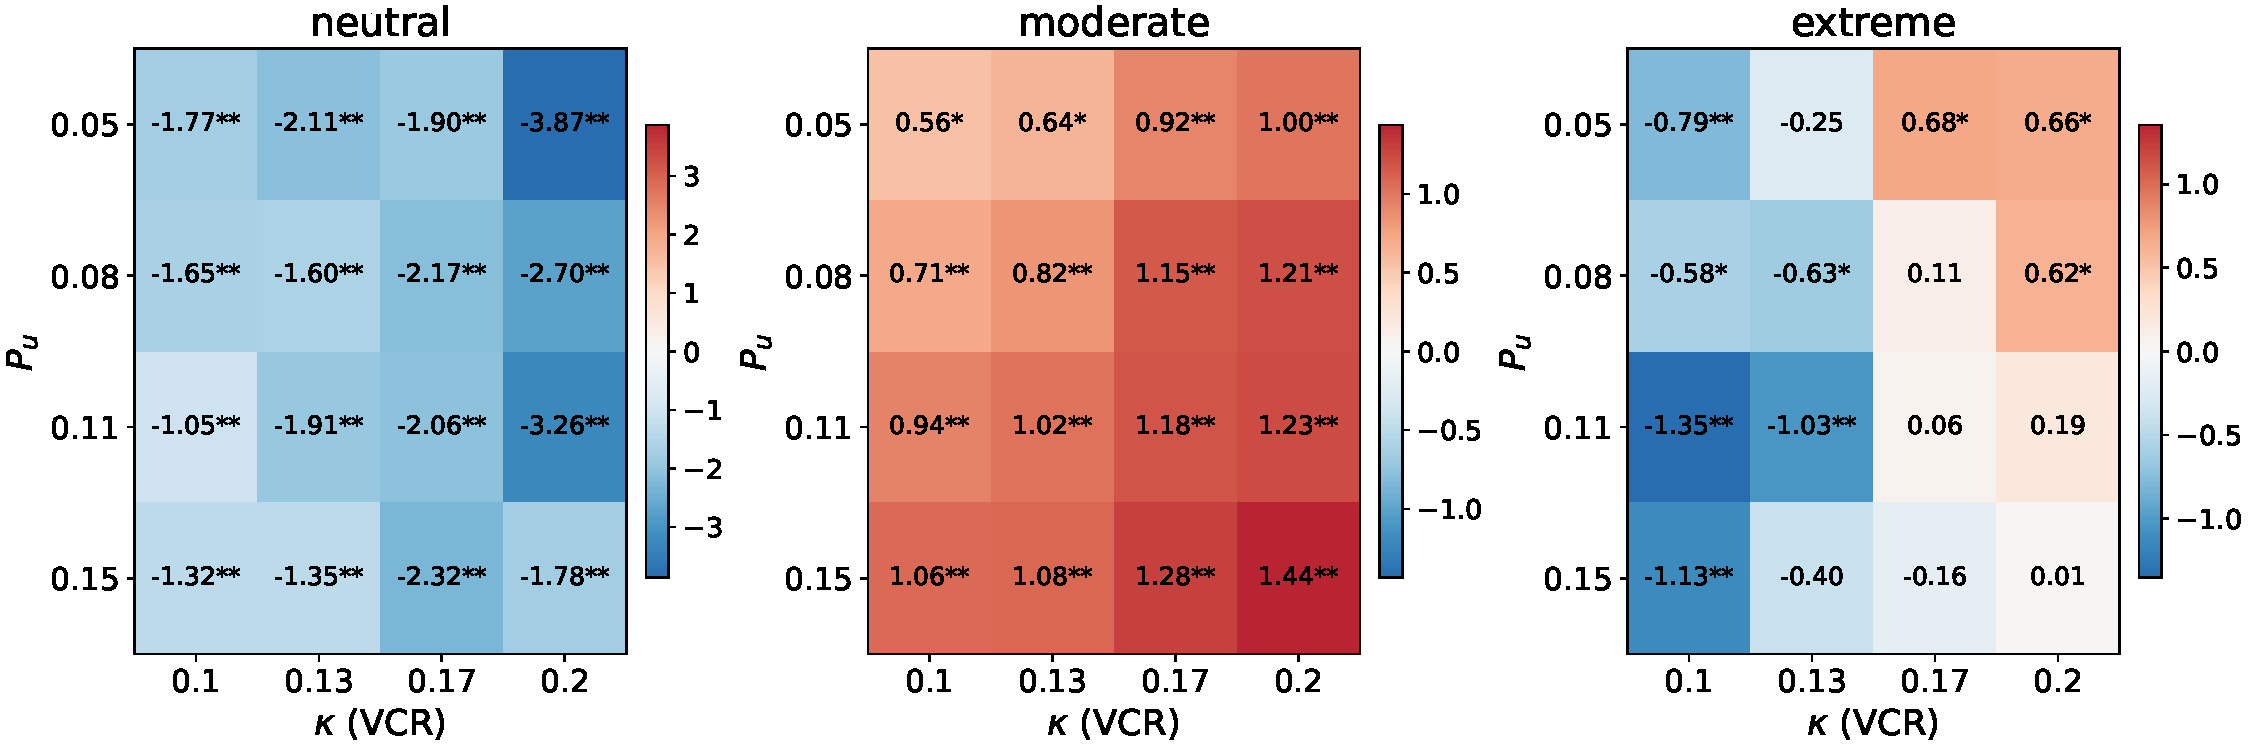
\includegraphics[width=\linewidth]{figures/outcome-heatmap.pdf}
\caption{Per-camp effect of moderate-hub silencing
on posting rate (M-silent -- control; paired Cohen's $d_z$ across seeds;
one-sided paired $t$-test: $*$~$p<0.05$, $**$~$p<0.01$)}
\label{outcome-heatmap}
\end{figure}

\begin{figure}[t]
\centering
\includegraphics[width=\linewidth]{figures/NE-E-influx.pdf}
\caption{Late trailing-window share of an extreme agent's feed
occupied by same-signed near-extreme-authored content:
for \emph{control} and \emph{M-silent}
(left, center), and their difference (right).}
\label{NE-E-influx}
\end{figure}

Fig.~\ref{outcome-heatmap} shows heatmaps of the paired
Cohen's $d_z$ (the mean seed-wise difference divided by its standard
deviation) in per-capita posting rate for each of
the three opinion camps, computed over the trailing window
$(38000, 40000]$, comparing \emph{M-silent} against
\emph{control}.
Steadily, the moderate camp boosts its posting
activity when it can perceive aligned-opinion
hubs' vocality, whereas the near-extreme camp
shrinks its posting by contrast.
Compared to these fairly intuitive results, the
extreme camp does not show a linear result: its
posting activity is reduced (a negative value in
the heatmap) when $\VCR$ is relatively low, for
each $P_u$ row, and it crosses the sign of its
effect at a different value of $\VCR$ depending on
the $P_u$ value.
Equivalently, reversing the contrast from
\emph{M-silent -- control} to \emph{control --
M-silent} lets us interpret the same difference
from the complementary perspective of the moderate
hub's activity rather than its absence. 
From this point of view, focusing on the presence
of moderate hubs, under the same propensity to
prune out-of-tolerance ties ($P_u$), moderate hubs
facilitate the extreme camp's posting activity
when agents speak only in the presence of
sufficient nearby agreement (low $\VCR$), and
suppress it in the opposite environment.

Also, $P_u$ can be interpreted as a modulator that
shifts the $\VCR$ cross-sign point, the watershed
value at which moderate hubs' vocality switches
between the facilitating and suppressing regimes
for the extreme camp.
In the extreme camp result of Fig.~\ref{outcome-heatmap},
the effect size in higher $P_u$ rows stays
negative across a wider range of low $\VCR$ before
turning positive at higher $\VCR$, compared with
lower $P_u$ rows.
This confirms that $P_u$ governs where this
sign reversal occurs.

Next, in order to see the upstream mechanism behind the
moderate hubs' cross-over role against extremes,
we investigated the interplay between near-extremes and
extremes.
Fig.~\ref{NE-E-influx} shows, for every condition, the trailing-window
share of an extreme agent's feed occupied by same-signed near-extreme-authored
content. This confirms that this share is steadily larger in
\emph{M-silent} conditions than in \emph{control} conditions.
This asymmetric influx difference between the two conditions,
shown in the rightmost panel, is mainly governed by $P_u$ and only
weakly by $\VCR$, growing several-fold as $P_u$ increases.

\section{Discussion}\label{sec:discussion}

The moderate and near-extreme camps -- whose posting activity
moderate hub vocalization amplifies and suppresses, respectively, a
pattern confirmed uniformly in Fig.~\ref{outcome-heatmap} -- are
well understood together, since both effects follow from the same
single mechanism. That is, posting probability, by construction
(Eq.~(\ref{eq:social-reinforcement})), depends on nothing other
than the fraction $c_i(t)$ of an agent's own feed that it currently
finds comfortable, thereby whichever camp's feed the moderate hubs' own
output reaches in substantial volume is the camp whose posting
behavior they move directly. The moderate camp is one such camp. 
Since a
moderate hub's opinion aligns with the moderate population's
opinion range, essentially almost every post that reaches a moderate
agent from a moderate hub falls within that agent's vocal comfort
radius $\VCR$. 
Moreover, moderate hubs supply the large majority of
the moderate-authored content the moderate population receives, thereby
silencing them drives a moderate agent's average feed-comfort
fraction from roughly $50\%$ down to roughly $30\%$, and its
posting activity down with it. The near-extreme camp is the second
such camp, but for the opposite direction. Moderate hubs occupy a
substantial share of a near-extreme agent's feed -- between roughly
$25\%$ and roughly $50\%$, depending on $P_u$ -- but their
opinion is too far from the
near-extreme camp's own opinion range to register as comfortable.
Activating moderate hubs therefore dilutes a near-extreme agent's
comfort ratio and suppresses its posting, while silencing them
removes that dilution and reactivates it.

The extreme camp's own result, however, cannot be explained by
either of the two direct mechanisms above, because 
a moderate hub's own
content comes to occupy no more than a few percent of an extreme
agent's feed. 
Quantifying this directly, the direct-removal arithmetic 
predicts a shift an order of magnitude too small
to explain the observed effect, 
confirming that the extreme camp's sign reversal must be a
downstream, ripple consequence of something other than
moderate-hub content reaching extreme agents directly.
We argue that this downstream effect operates through
two layers: an \emph{openness} layer (the homophily-driven gating
introduced above) that determines how much near-extreme content
reaches the extreme camp, and a \emph{comfort} layer (its
spiral-of-silence-style counterpart) that determines how the arriving
content is evaluated. The two layers operate sequentially: openness
determines what an extreme agent is exposed to, after which comfort
determines whether that content is experienced as supportive or
disruptive.

The openness mechanism is governed by $P_u$, and it operates through
$\BoundedConfidence_i(t)$ rather than around itself. Since a tie 
is newly formed or severed 
through $\BoundedConfidence_i(t)$, the width of an extreme agent's
own bounded-confidence threshold is what decides whether a
near-extreme author is eligible to be followed and retained, or is
instead blocked. Crucially, 
this gating against the near-extreme is not processed uniformly, 
a narrow
$\BoundedConfidence_i(t)$ admits only its \emph{extreme-ward} edge
while a wider $\BoundedConfidence_i(t)$ extends
admission toward its \emph{moderate-ward} edge.
% Therefore, $\BoundedConfidence_i(t)$ gates not only how much
% near-extreme content is admitted, but how far into the near-extreme
% range an agent admits. 
At this point, we introduce the fact 
that a higher $P_u$ is associated
with a wider converged $\BoundedConfidence_i(t)$ among extreme
agents, which is confirmed as
a monotonic trend within every individual $\VCR$ stratum
(Kendall's $\tau=0.29$--$0.38$, $p<10^{-4}$ in each stratum).
This pattern arises as follows:
first, $\BoundedConfidence_i$ is low in the opening steps regardless of
$P_u$, because agents are more likely to be exposed to out-of-tolerance
content before they have severed ties with such sources. 
From this low
starting point, agents gradually recover $\BoundedConfidence_i$ as
they finish unfollowing or blocking distant sources, 
therefore, 
a higher $P_u$ lets that recovery
converge to a wider $\BoundedConfidence_i(t)$ 
by pruning those sources faster. 
Moreover, the
difference in near-extreme post volume reaching an extreme agent's
feed between the two conditions(Fig.~\ref{NE-E-influx}) grows consistently with $P_u$,
supporting the \emph{openness} role of $P_u$
through $\BoundedConfidence_i$. As a direct network-level check on
this account, the \emph{M-silent}$-$\emph{control} gap in the mean 
number of directed edges from an extreme agent to 
same-sign near-extreme agents at $t=40{,}000$ itself grows
with $P_u$ (from $+0.08$ at $P_u=0.05$ to $+0.22$ at $P_u=0.15$, a
$1.3\times$-to-$2.4\times$ ratio), directly confirming, at the level
of the follow graph, the same pattern
Fig.~\ref{NE-E-influx} shows in terms of feed exposure.

The comfort mechanism, by contrast, is governed by $\VCR$ itself. 
Whatever near-extreme content the openness
mechanism admits, $\VCR$ then determines the evaluation of that
content in a way comfortable if within $\VCR$.
This evaluation role of $\VCR$ lets it fix
the direction of the extreme
camp's sign reversal: under a narrow $\VCR$, few of the
admitted near-extreme content falls inside the comfort range, thereby
admission only dilutes the comfort ratio and posting moves
downward; under a wide $\VCR$, a non-trivial share does fall inside
the comfort range, thereby posting moves upward instead. In other words,
under the same $P_u$, silencing moderate hubs deactivates extreme
posting when $\VCR$ is low, and activates it when $\VCR$ is high. 
As shown in Fig.~\ref{outcome-heatmap},
this sign-change point shifts toward higher $\VCR$ as $P_u$
increases, because the wider $\BoundedConfidence_i(t)$, resulting from 
higher $P_u$, retains \emph{moderate-ward} near-extreme sources, 
thereby a wider $\VCR$ is
needed before their content registers as comfortable. Notably, the
effect is relatively small at high $\VCR$ and high $P_u$ in
Fig.~\ref{outcome-heatmap} since the wider $\BoundedConfidence_i$ 
admits more comfortable near-extreme content,
but more uncomfortable near-extreme content alongside it, 
partly canceling each other. 

To capture the effect of an \emph{active} moderate hub specifically,
we restate the mechanism above as complementary to the silencing 
context so far. 
The negative region
of Fig.~\ref{outcome-heatmap} is the facilitating regime, where an
active moderate hub boosts extreme posting; the positive region is
the suppressing regime, where it suppresses extreme posting. In the
facilitating regime ($\VCR$ low), the disruptive near-extreme
content that would otherwise arrive under \emph{M-silent} simply
does not arrive, thereby the extreme camp's feed stays comfortable. In
the suppressing regime ($\VCR$ high), it is instead the 
(extreme-ward edge) near-extreme
content which $\BoundedConfidence_i(t)$ would have admitted as such 
satisfying $\VCR$ that fails to arrive, thus, the extreme camp loses a
source of comfortable content it would otherwise have had. 
Again, the flipping point of $\VCR$ is adjusted by $P_u$. 
Therefore,
viewed through the lens of posting activity, an active moderate hub
acts less as a conduit than as an upstream regulator.

\section{Conclusion}\label{sec:conclusion}
In this study, we investigate how activating or silencing 
moderate hubs shapes vocalization dynamics in a 
social-media-inspired ABM on a heavy-tailed follow network. 
We find that moderate hubs exert direct, opposing 
effects on moderate and near-extreme populations 
through the comfort of their feed exposure. 
They amplify posting among aligned moderate agents 
while suppressing it among near-extreme agents. 
In contrast, their effect on extreme agents is indirect 
and inconsistent, 
arising through changes in near-extreme content flow. 
This downstream effect is governed by two 
layered mechanisms: openness, which determines 
which near-extreme content reaches extreme agents; 
comfort, which determines how that content 
affects their posting. 
As a result, the effect of moderate-hub activity 
on extreme posting can reverse across parameter regimes. 
These findings suggest that, at least from the vantage point of
vocalized activity, moderate hubs should not
be understood simply as bridges that connect otherwise
distant camps in social media, but as upstream
regulators whose activity reshapes the information
environment and can produce ripple effects downstream.
Crucially, this interpretation is conditional on the model's
assumptions about adaptive exposure, comfort-driven
posting, and a single-dimensional opinion representation. Whether the observed sign reversal generalizes
beyond these assumptions and occurs in empirical settings 
remains an open question for future work.

\bibliographystyle{spmpsci}
\bibliography{refs}
\end{document}
